\chapter{Experimental Setup }

\section{Founding and History}

\section{Large Hadron Collider}

\begin{figure}
\begin{center}
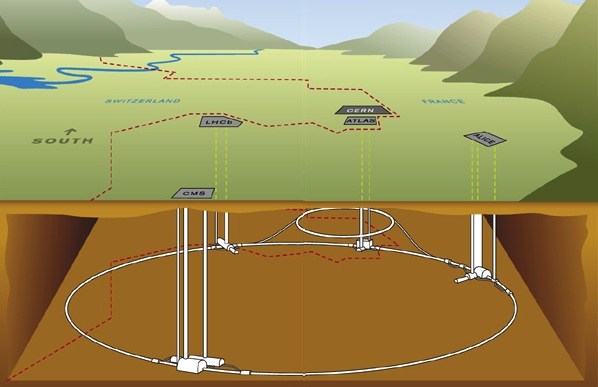
\includegraphics[width=.5\textwidth]{lhc_tunnel}
\caption{The LHC tunnel installed on the border of Geneva, Switzerland and France. 
The experiments are distributed along the circumference of the ring.}
\end{center}
\end{figure}

The bunches of protons in the LHC are bent into a circular trajectory by more than 1200
 superconducting dipole magnets and are focused and maintained close to the ideal
 orbit around the ring by hundreds of superconducting quadrupole magnets. 
Thousands of corrector magnets around the ring allow the beam to be steered closer 
to the ideal orbit, make the focusing independent of the particles’ energy variations
 within a bunch, and cancel the effects of higher order multipoles in the fields induced 
by small field imperfections in the main magnets. 
The radiofrequency (RF) field in superconducting cavities is placed periodically around 
the ring and accelerates the protons from the injection energy of 450 GeV to the final
 operating energy, which is designed to be 7 TeV per beam. The RF field also causes the
 protons to be bunched, as only particles at or near a certain ”equilibrium phase” on 
the RF wave will be accelerated stably. Special quadrupoles around each interaction region
 focus the bunches down to a small transverse size, to increase the likelihood of a
 proton-proton collision each time two bunches pass through each other.

\section{Other LHC Related Experiments}

\section{Compact Muon Solenoid Experiment}

\begin{figure}
\begin{center}
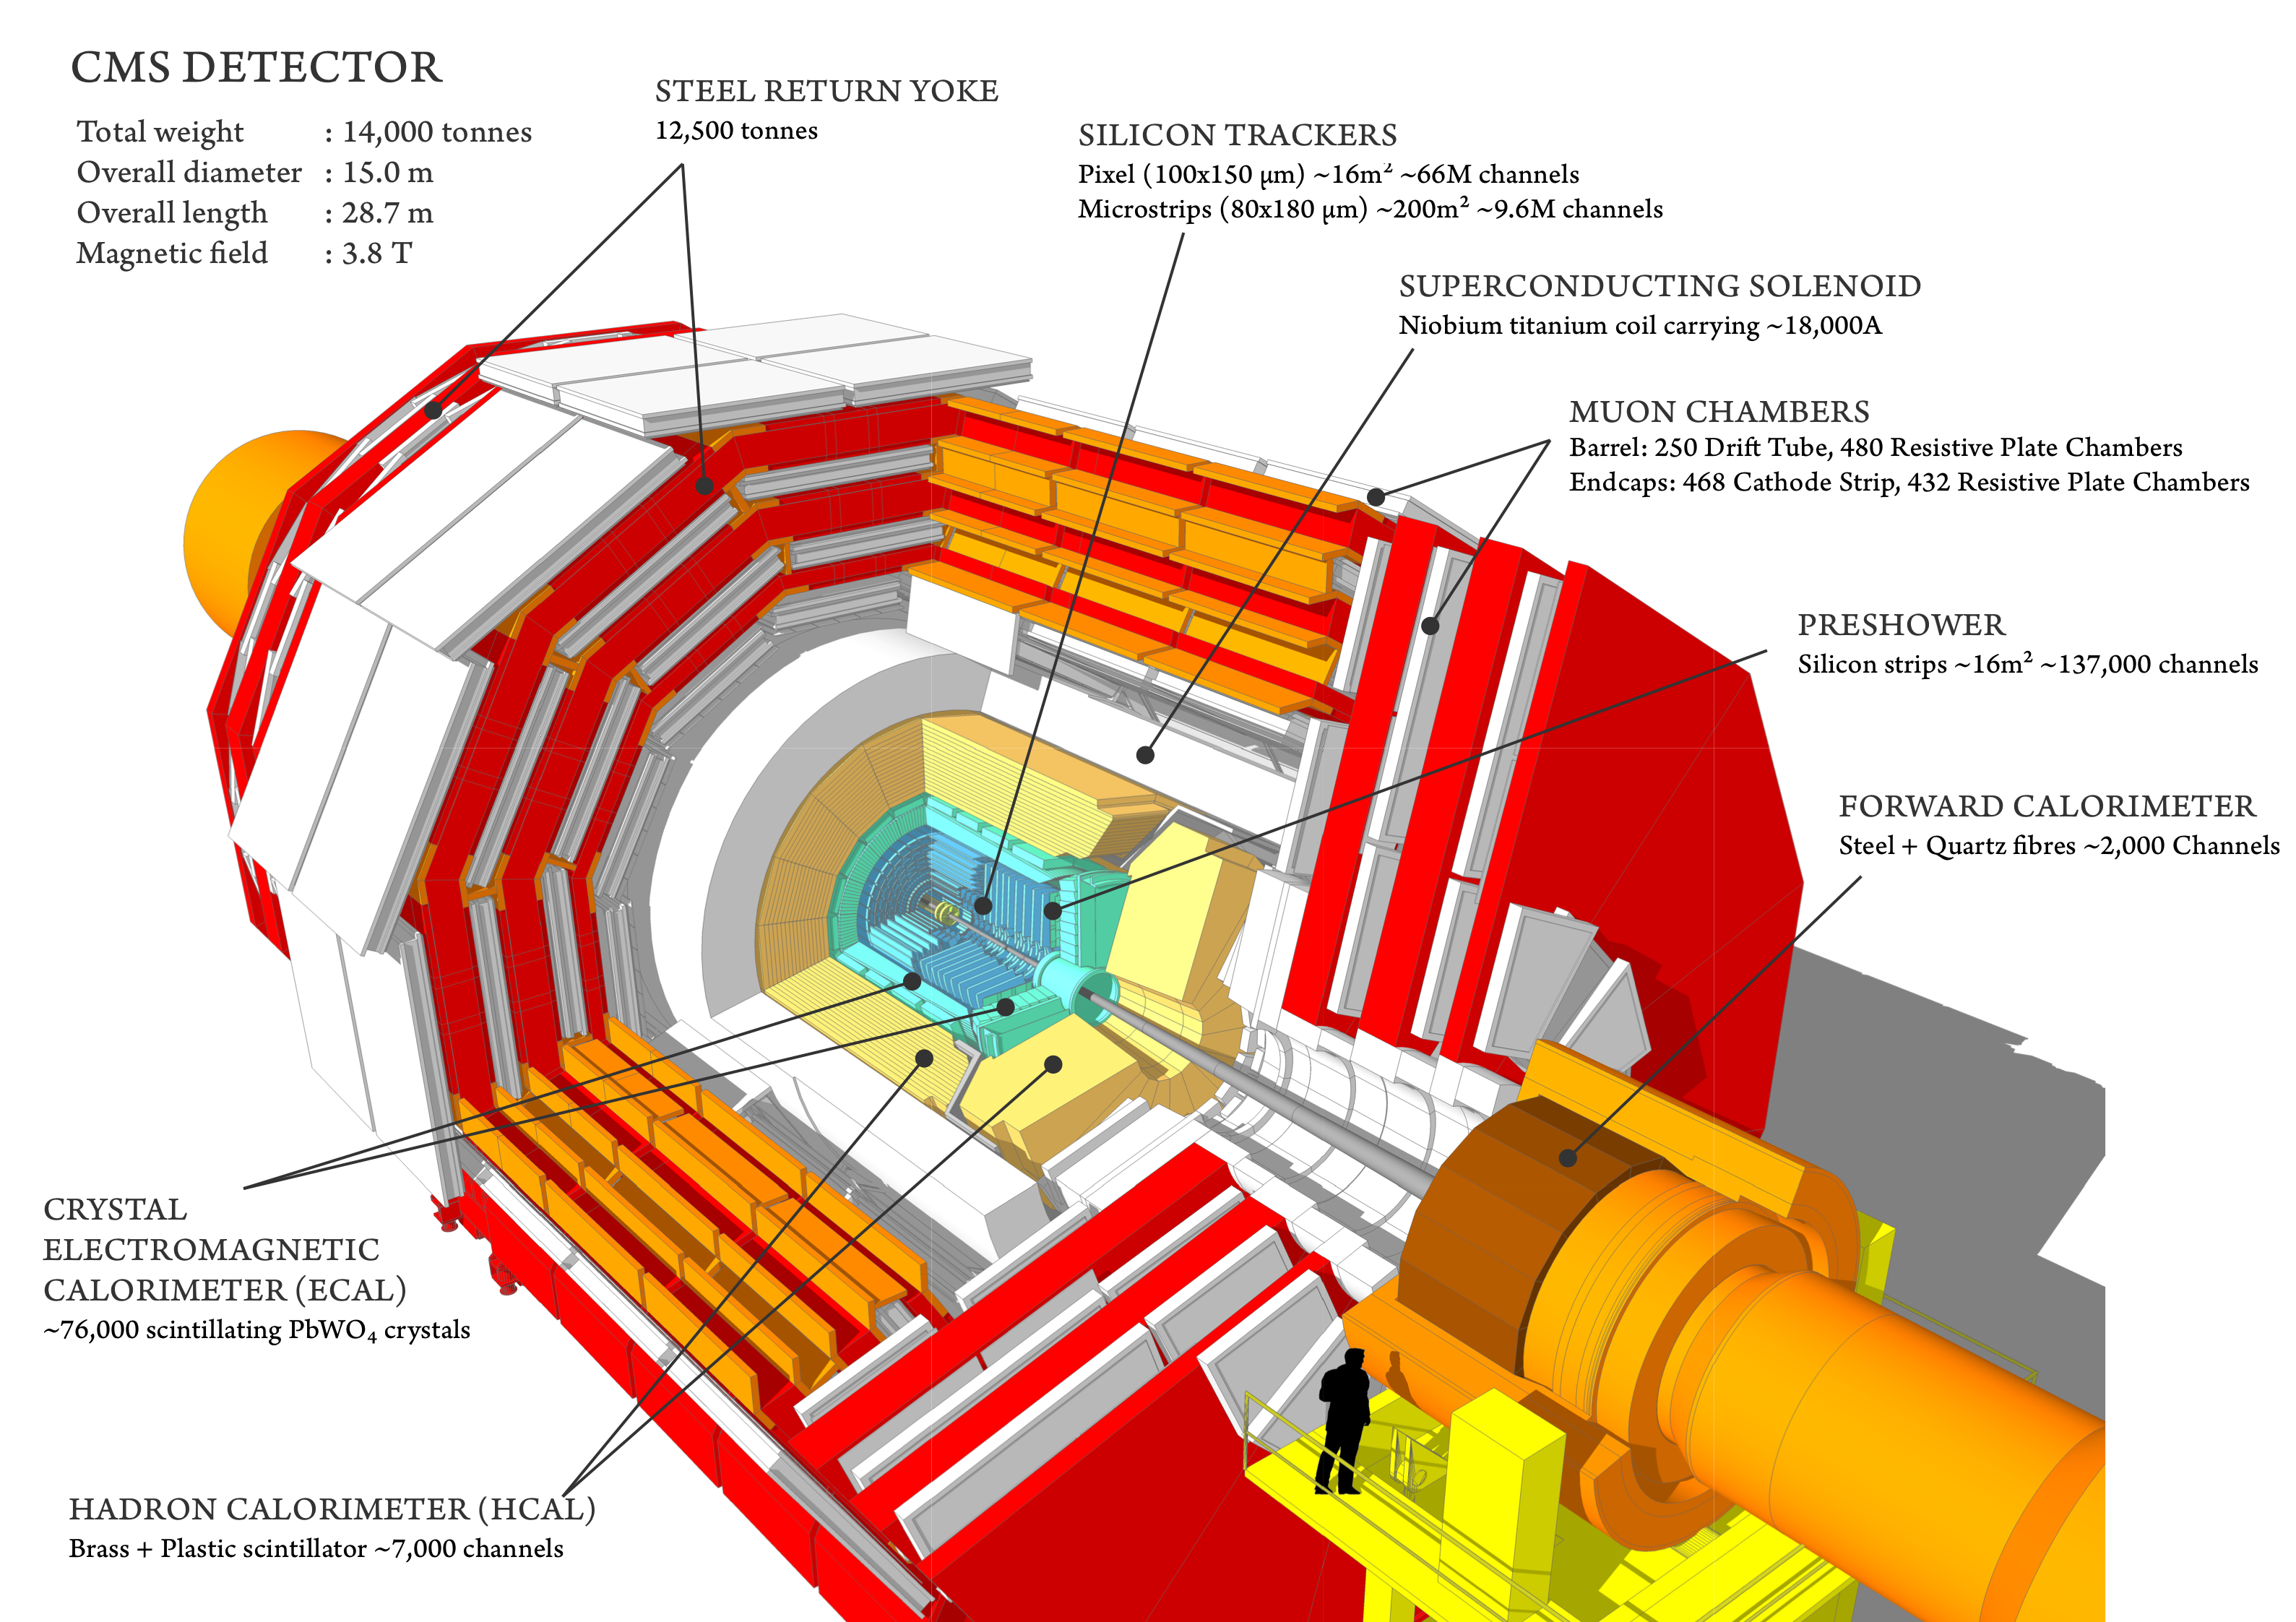
\includegraphics[width=.55\textwidth]{figures/pre_thesis/cms.png}
\hspace{.1in}
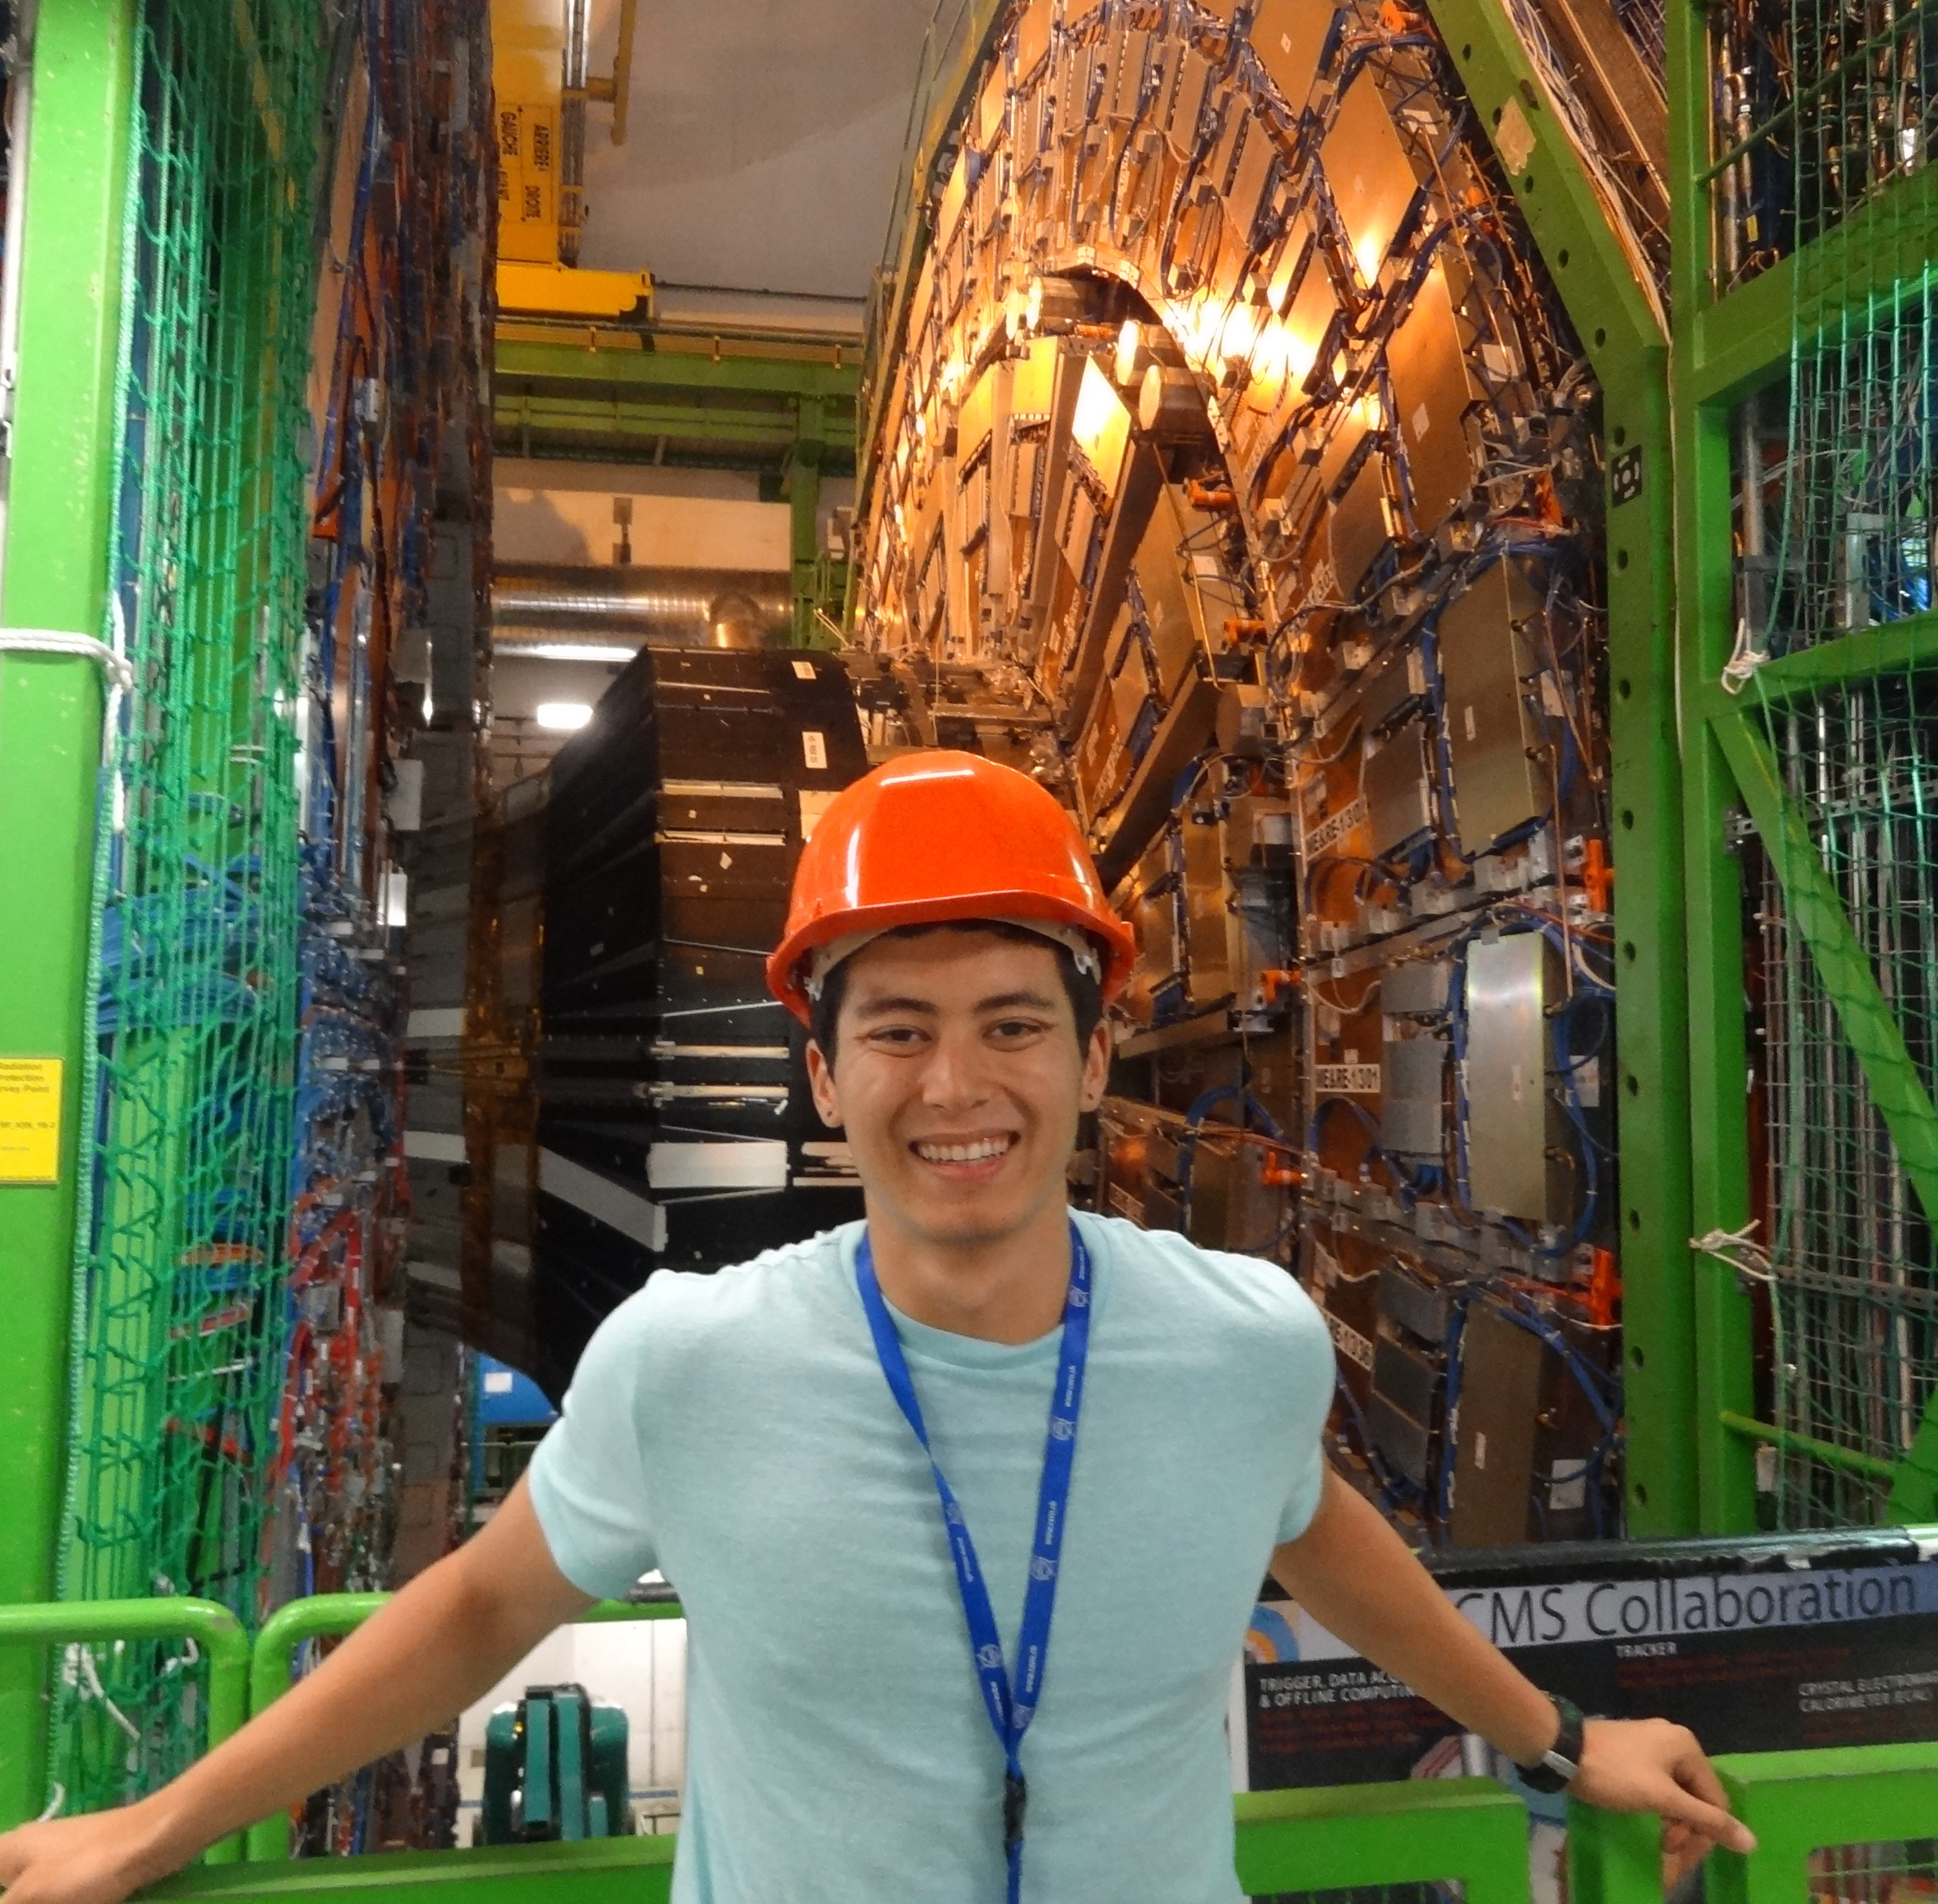
\includegraphics[width=.4\textwidth]{figures/pre_thesis/selfie}
\end{center}
\caption{(left) A tear-away view of the inner detectors of CMS. (right) The CMS endcap currently detached from the inner barrel for upgrades during the shutdown.}
\label{fig:cms}
\end{figure}

The Compact Muon Solenoid (CMS) Detector is a general-purpose detector consisting of 
an all silicon tracker, a precision electromagnetic calorimeter (ECAL), a hadron calorimeter
 (HCAL), a 4 T superconducting solenoid and muon chambers. The solenoid deflects charged
 particles whose paths are traced in the tracker, making it possible to 
reconstruct the particles’ momentum. The two calorimeters reconstruct the energy 
of and identify photons, electrons and hadronic jets.
As shown in Figure \ref{fig:cms} the detector has cylindrical symmetry about the
 interaction point where the proton beams collide. By maintaining near full coverage 
of the interaction point it is possible to detect signatures such as neutrinos or other weakly interacting particles as missing energy. 


\subsection{ECAL}

\subsection{HCAL}

\subsection{Tracking}

\begin{figure}
\begin{center}
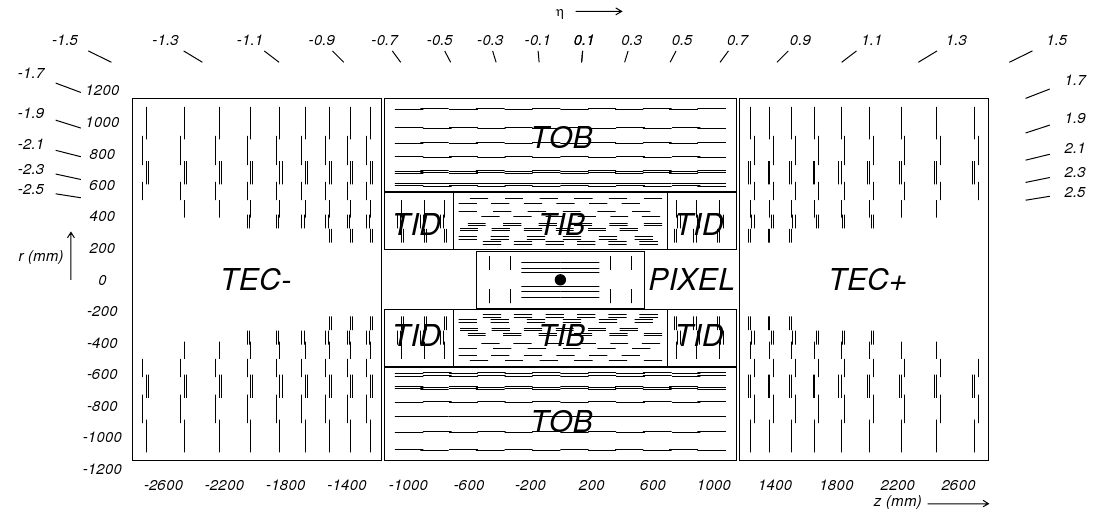
\includegraphics[width=.9\textwidth]{figures/an_jetid/DETECTOR/cms_tracker}
\end{center}
\caption{The CMS Tracker}
\label{fig:tracker}
\end{figure}

\subsection{Muon Chambers}

\subsection{Trigger System}

\begin{figure}
\begin{center}
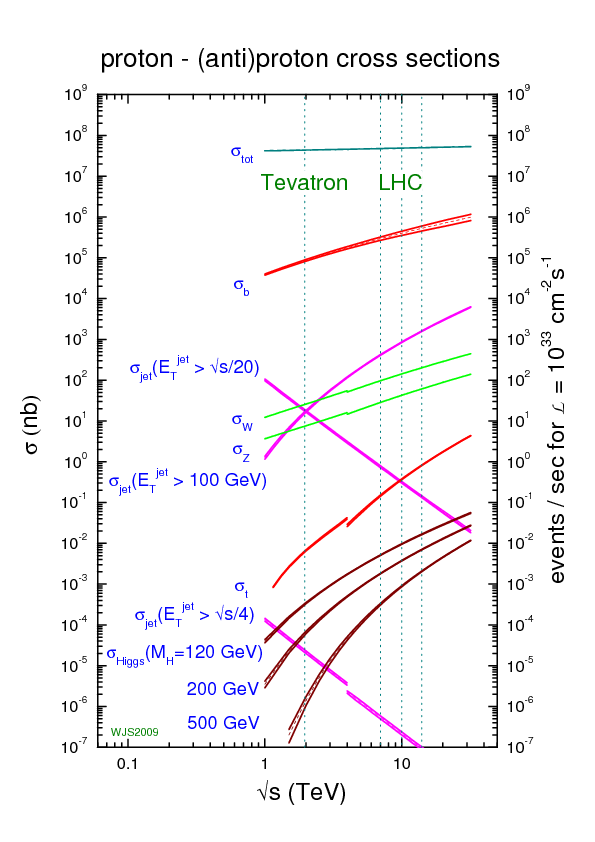
\includegraphics[width=2.9in]{figures/exp_proj/pdf_xsec.png}
\caption{Common cross sections of proton collisions as a function of the center of mass energy $\sqrt{s}$}
\end{center}
\label{fig:pdf_xsec}
\end{figure}

The CMS Trigger System exists as a filter through which events are determined to be ``interesting''. 
It is both  unnecessary and inefficient to record anything that occurs in the detector electronics. 
Most events that occur from colliding protons are well understood. To the left, you can see the 
logarithmic plot of common physics processes for proton-proton scattering. Events such as the production 
of a $b$ quark  occur at $\approx 10^6$ Hz at a luminosity of $\mathcal{L} = 10^{33}$ cm$^{-2}$ 
whereas the production of the Higgs is much lower at $\approx 10^{-2}$ Hz.  \\

At design luminosity, the LHC has beam crossings at a rate of $\approx 40$ MHz with 
each crossing coming spaced at $\approx$ 25 ns. 
For each crossing there are $\approx$ 20 inelastic collisions (referred to as pile up) 
contained in an event file of $\approx$ 1 Mb. 
However the bandwidth for storage is limited to $\approx 10^2$ Hz and equivalently $10^2$ Mb/s. 
Generally, all but one of the inelastic collisions is interesting and a large excess of uninteresting 
activity is generated in the detector electronics. The trigger must be robust enough to select 
this needle in a haystack event while remaining computationally efficient in maximizing the limited bandwidth.  \\

The CMS Trigger system is designed to read events at the event crossing frequency and generate the
 factor $10^5$ of rejection between the crossing frequency and the archival capacity. This factor 
is far too large to achieve in a single step given the complexity of triggers and event reconstruction. 
Therefore the task is split into two steps: The Level 1 (L1) and High Level (HLT) Trigger systems.

The $O(10^7$) events per second first pass through the L1 Trigger which reads out events at $10^5$ Hz. 
From here, the High Level Trigger makes the final decision as to which events are kept. 
Approximately 350 Hz is processed and stored, 300 Hz is ``parked'' (stored but processed later), 
and 1 kHz is partially stored (only the HLT level information and not the RAW detector information) 
and used for data scouting for future analysis.  \\

The most basic criterion for interesting events are hard physics events with high momentum transfer, $q^2$.
 As the protons collide with effectively no transverse momentum, any event with significant deposits of 
transverse energy (or even missing transverse momentum) is indicative of a hard physics process. 
The number of objects with a given transverse momentum falls off exponentially, so a simple minded way to
  reduce the rate of processed events is to raise the threshold of accepted events. \\

More specific criterion for ``interesting events'' is analysis dependent. Generally, analyses are
 categorized by their final state signature. Thus, the trigger requires loose identification 
on the objects of that signature such as the isolation and shape of energy deposition. 
Once the event has passed the Level 1 and HLT Triggers, tighter and more computationally 
costly selection can be made offline where we are unrestricted by bandwidth limitations. \\

As there is a limited amount of bandwidth for processing the events, the numerous analyses of CMS
 are given a budget (measured in Hz) for the triggers they request. As it stands the $H\rightarrow \gamma\gamma$ 
analysis is assigned a budget of 30 Hz for its diphoton trigger suite. As the diphoton channel was of 
high priority in the 7 and 8 TeV running this accounted for a significant fraction ($\approx$10\%) of the overall budget. \\

As the luminosity of the machine increases, we expect proportionally more events per second and must accordingly alter the triggers. 

\begin{figure}
\begin{center}
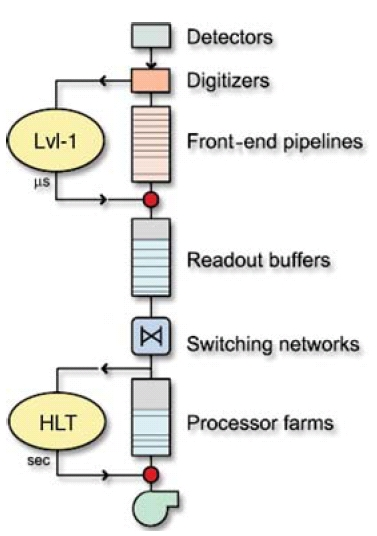
\includegraphics[width=2.5in]{figures/exp_proj/cms-trigger}\\
\caption{A diagrammatic representation of the level 1 and HLT trigger processing}
\end{center}
\end{figure}


\subsubsection{Level 1 (L1) Trigger}

\subsubsection{High Level Trigger (HLT)}

